\documentclass{beamer}
\usepackage{amsmath}
\usepackage{wrapfig}
\usepackage{enumerate}
\usepackage[makeroom]{cancel} % ������������
\usepackage{multicol,multirow} %��������� �������
\usepackage{hyperref}
\usepackage{tabularx}
\usepackage{amsfonts}
\usepackage{amssymb}
\usepackage{amsmath}
\DeclareMathOperator{\Tr}{Tr}
\DeclareMathOperator{\diag}{diag}
\DeclareMathOperator{\conv}{conv}
\DeclareMathOperator{\Rg}{Rank}
\DeclareMathOperator{\Ker}{Ker}
\newcommand{\matrixl}{\left|\left|}
\newcommand{\cbad}{c_{\mathrm{bad}}}
\newcommand{\matrixr}{\right|\right|}
\DeclareMathOperator*{\argmin}{arg\,min}
\newcommand{\h}{\mathbf{h}}
\newcommand{\x}{\mathbf{x}}
\newcommand{\aaa}{\mathbf{a}}
\newcommand{\w}{\mathbf{w}}
\newcommand{\W}{\mathbf{W}}
\newcommand{\y}{\mathbf{y}}
\newcommand{\X}{\mathbf{X}}
\newcommand{\Y}{\mathbf{Y}}
\newcommand{\fx}{\mathbf{f}}
\newcommand{\fs}{\mbox{f}}
\usepackage[cp1251]{inputenc}
\usepackage[russian]{babel}
\usepackage{amsmath,mathrsfs,mathtext}
\usepackage{graphicx, epsfig}
\usetheme{Warsaw}%{Singapore}%{Warsaw}%{Warsaw}%{Darmstadt}
\usecolortheme{sidebartab}
\definecolor{beamer@blendedblue}{RGB}{55,172,32}
%----------------------------------------------------------------------------------------------------------
\title[\hbox to 56mm{Power Flow Feasibility problem  \hfill\insertframenumber\,/\,\inserttotalframenumber}]
{Power flow feasibility problem}
\author[S.E. Volodin]{\large \\Sergei Volodin\\under supervision of Y. Maximov}
\institute{\large Skolkovo Insitute of Science and Technology}

\date{}
%-------------------------------------------------------
\begin{document}
%-------------------------------------------------------
\begin{frame}
%\thispagestyle{empty}
\titlepage
\end{frame}
%-------------------------------------------------------
\begin{frame}{The problem}
\begin{enumerate}
\item Large-scale power grids
\item Need to know if a regime of the grid is <<normal>>, <<safe>>
\item Ohm's law $\Rightarrow$ quadratic equations:
$$y_i=f_i(x)=x^TA_ix+2b_i^Tx$$
$y$ (regime) known, $x$ is not
\item Need to determine if $\exists x\colon y=f(x)$ (means <<safe>>)
\end{enumerate}

This problem is known as Power Flow Feasibility problem.

To solve it, the image $f(\mathbb{R}^n)$ must be examined
\end{frame}

\begin{frame}{State of the art}
\begin{enumerate}
\item A. Dymarsky, Convexity of a Small Ball Under Quadratic Map, arXiv:1410.1553
\item A. Dymarsky, On the Convexity of Image of a Multidimensional Quadratic Map, arXiv:1410.2254
\end{enumerate}
\end{frame}

\begin{frame}{The solution}
Given: the map $f\colon\mathbb{R}^n\to\mathbb{R}^m$, $f_i(x)=x^TA_ix+2b_i^Tx,\,A_i^T=A_i$
Proposed algorithm for examining $F=f(\mathbb{R}^n)$:
\begin{itemize}
\item {\bf Input:} $y^0\in F$, direction $c_+\colon c_+\cdot A>0$
\item {\bf Output:} value $z_{\max}$ s.t. the cut $Q(c_+,z_{\max}, F)$ is convex
\end{itemize}
$$Q(c_+,z,F)=\{y\big| (y-y^*,c_+)\in[0,z]\}\cap F$$\\
\vspace{30px}
\centering 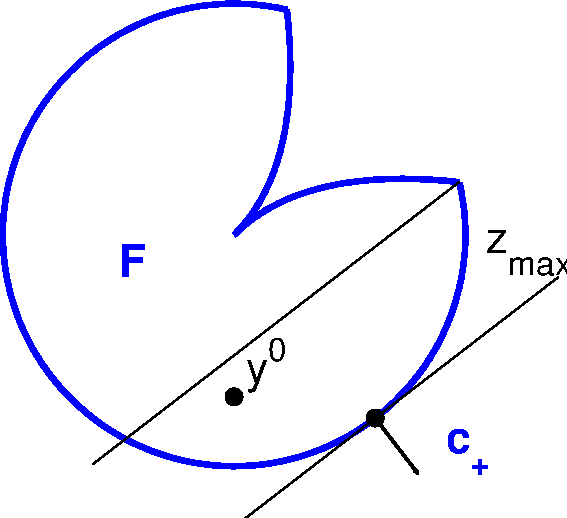
\includegraphics[width=100px]{cut}\\
\centering $y^*$~--- touching point of hyperplane $c_+$\\
\end{frame}

\begin{frame}{The solution}
The idea of the algorithm:
\begin{enumerate}
\item Discovering boundary nonconvexities $\{F_i\}$ close to $y^0$
\item Projecting to $c_+$: $(F_i,c_+)$
\item Calculating $z_{\max}=\inf\limits_i \inf\limits_{y\in F_i}(c_+,y)$
\end{enumerate}
\vspace{30px}
\centering 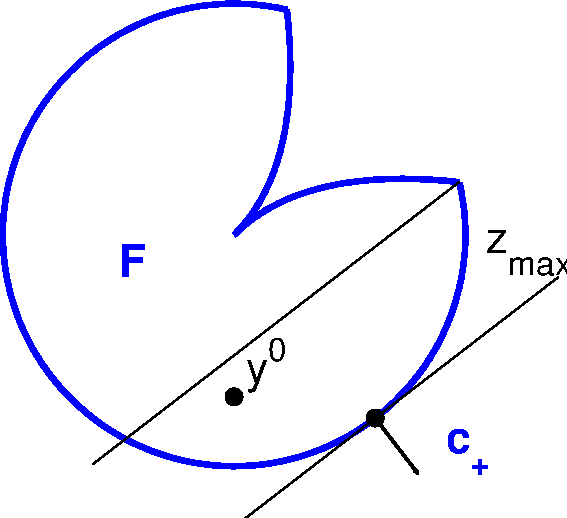
\includegraphics[width=100px]{cut}
\end{frame}

\begin{frame}{The solution}
	Boundary points of F on supporting hyperplane $c$:
	$\partial F_{c}=f(\argmin\limits_{x\in\mathbb{R}^n}(c,f(x)))=f(\Ker (c\cdot A)-(c\cdot A)^g(c\cdot b))$
	
	$$\mbox{if }\begin{cases}
	c\cdot A\geqslant 0\\
	(c\cdot b)^T\Ker (c\cdot A)=0
	\end{cases},\,\mbox{otherwise }\partial F_c=\emptyset$$
\begin{itemize}
\item $\partial F_{c}$ is nonconvex $\Rightarrow$ $F$ has nonconvexity
\item $\partial F_c$ is nonconvex $\Leftrightarrow^{(*)}$ $\Rg (c\cdot A)=n-1$, $c\cdot A\geqslant 0$
\end{itemize}
Therefore, $$z_{\max}=\inf\limits_c\inf\limits_{y\in \partial F_c} (c_+, \partial F_c)$$\\
(*) {\em We assume $\Rg(c \cdot A)< n-1$ to be a rare case. Condition $\Rg (c\cdot A)=n-1$ is associated with nonconvexity of $\partial F_c$}
\end{frame}

\begin{frame}{The solution}
Linear change of basis s.t.
$\begin{cases}
c_+\cdot A=I,\,c_+\cdot b=0
\end{cases}$ $\Rightarrow$
\begin{itemize}
\item $\inf\limits_{y\in \partial F_c} (c_+, \partial F_c)=\|(c\cdot A)^g(c\cdot b)\|^2$ for $c\colon \Rg (c\cdot A)=n-1$
\item Adding $\gamma c_+$ to $c$ to ensure $\lambda_{\min}\big((c+\gamma c_+)\cdot A\big)=0$\\
{$c_+\cdot A=I$ by our choice of variables}
\item Define $z(c)=\|(c\cdot A-\lambda_{\min}(c\cdot A))^g(c\cdot b)\|^2$
\item Define $\cbad=\{c\big| \Ker(c\cdot A)\bot (c\cdot b)\}$\\
{\em $c\in\cbad\Leftrightarrow$ $z(c)$ has its original meaning, useless otherwise}
\item Then $$\boxed{z_{\max}=\inf\limits_{c\in\cbad}z(c)}$$
\item In general case $|\cbad|$ is continuum
\end{itemize}
\end{frame}
\begin{frame}{The solution}
We use gradient projection method to find
$$z_{\max}=\inf\limits_{c\in\cbad}z(c)$$
\begin{enumerate}
	\item {\bf Input:} start point obtained via {\em nonconvexity certificate}
	$$c^0\in\cbad$$
	\item Gradient $\frac{dz}{dc}$ is calculated explicitly
	\item Normal vector $n$ for $\cbad$
	\item Projection of $c'$ onto $\cbad$ is done by adjusting $\lambda$ in $c'+\lambda n$
	\item Repeat until $\frac{dz}{dc}\parallel n$
	\item {\bf Output:} minimal value $z_{\max}=z(c^*)$
\end{enumerate}
\end{frame}

\begin{frame}{The solution}
\begin{minipage}{1\textwidth}
	\centering Nonconvexity certificate:
\end{minipage}
\begin{wrapfigure}{l}{0.4\textwidth}
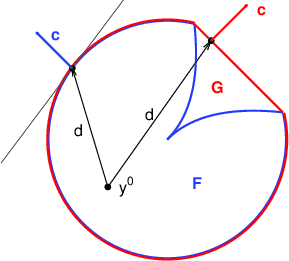
\includegraphics[width=100px]{alg_idea20}
\end{wrapfigure}
\begin{enumerate}
\item {\bf Input:} $y^0$
\item Generating random directions $d$
\item Find $t\colon y^0+td\in\partial \conv F$
\item $y^0+td\in F$?
\item If not, obtain $c$ via dual problem
\item {\bf Output:} <<nonconvex>> $c\in\cbad$
\end{enumerate}
\vspace{20px}
\hspace*{-100px}
$\Rightarrow$ Obtained start point for gradient descent
\end{frame}

\begin{frame}{The solution}
\centering
Gradient step + projection
\begin{tabular}{cc}
\begin{minipage}{0.5\textwidth}
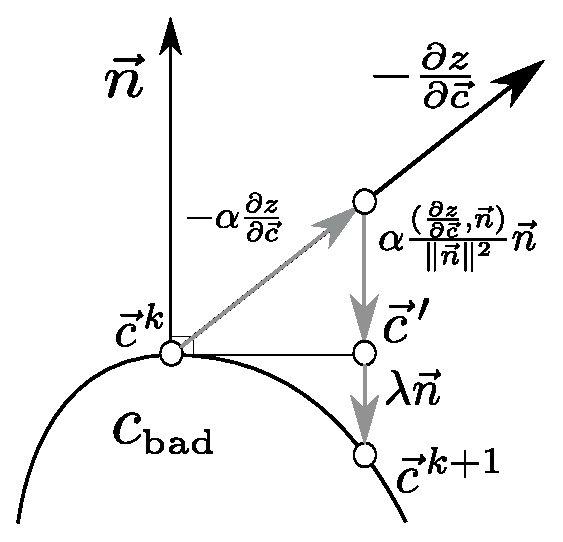
\includegraphics[width=150px]{c_bad_continuum}
\end{minipage} &

\begin{minipage}{0.5\textwidth}
\begin{enumerate}
	\item {\bf Input:} current point $c=c^k\in\cbad$
	\item Calculate $n(c)$, $\frac{dz}{dc}$, $c'=c-\alpha(\hat{1}-\frac{(\cdot, n)}{(n,n)}n)\frac{dz}{dc}$
	\item Project $c'\notin \cbad$ onto $\cbad$
	\item {\bf Ouput:} $c^{k+1}$ $\leftarrow$ result of projection
\end{enumerate}
	\end{minipage}
\end{tabular}
\end{frame}

\begin{frame}{The solution}
Projection

{\bf Given:} point $c'\notin \cbad$, normal vector $n$\\
{\bf Find:} point $c\in\cbad$ close to $c$
\begin{enumerate}
	\item $c(\lambda)=c'+\lambda n$
	\item For some $\lambda$, $c(\lambda)\in \cbad$
	\item $c(\lambda)\in \cbad$ $\Leftrightarrow$ $\Ker(c(\lambda)\cdot A)\bot c(\lambda)\cdot b$
	\item $m(\lambda)=(c(\lambda)\cdot b)^Tx_0(\lambda)$, $x_0(\lambda)\in\Ker (c(\lambda)\cdot A)$
	\item Projection is done by finding root of $m(\lambda)$
	\item Bisection method is used
\end{enumerate}
\end{frame}
\begin{frame}{Numerical experiment}
$f\colon \mathbb{R}^4\to\mathbb{R}^4$
\begin{itemize}
\item 4 local minima
\item Global minimum found
\end{itemize}
\centering 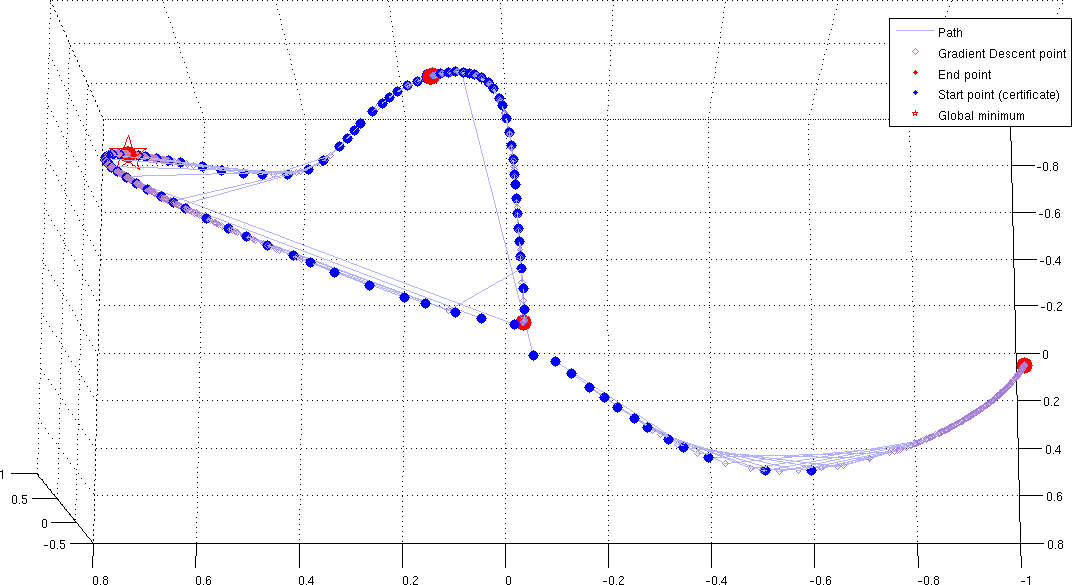
\includegraphics[width=300px]{example03_cbad_91pts_03.png}
\end{frame}

\begin{frame}{Results}
Algorithm for examining the set of <<safe>> regimes was proposed:
\begin{enumerate}
\item Can determine if the whole subset is <<safe>> at one run
\item Cuts convex parts of the image $F$
\item General case when the set of nonconvexities is a continuum was considered
\item Algorithm was tested on a number of maps $f$
\end{enumerate}
Plan:
\begin{enumerate}
	\item What happens to $\cbad$ if $\Rg(c\cdot A)=n-2$?
	\item $\mathbb{C}$ case
	\item Testing for $n,m>4$
	\item Testing for $n,m\gg1$
\end{enumerate}
%\vspace{40px}
\begin{tabular}{cccc}
\begin{minipage}{0.23\textwidth} 
\hspace*{-30px}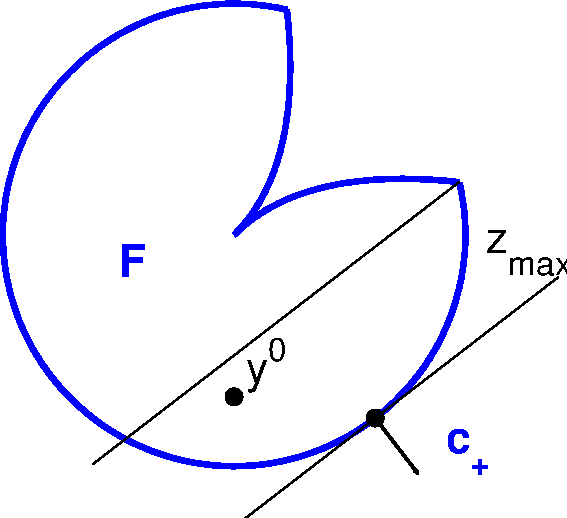
\includegraphics[height=60px]{cut}
\end{minipage} &
\begin{minipage}{0.23\textwidth}
\hspace*{-40px}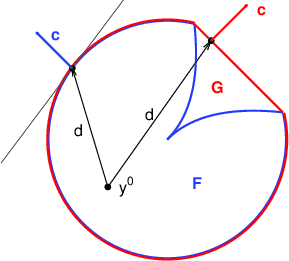
\includegraphics[height=60px]{alg_idea20}
\end{minipage} &
\begin{minipage}{0.23\textwidth}
\hspace*{-35px}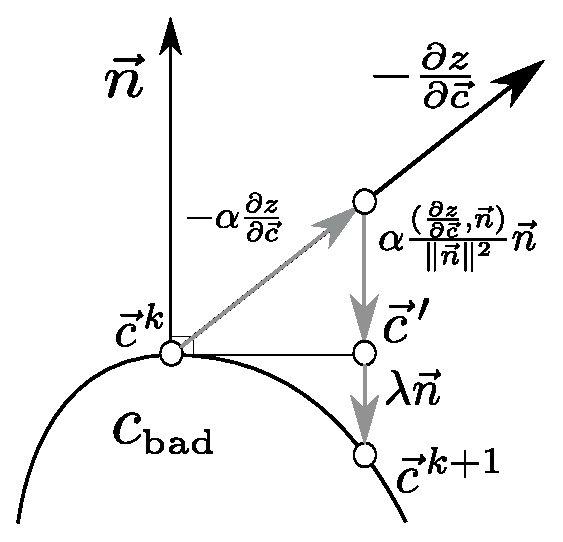
\includegraphics[height=60px]{c_bad_continuum}
\end{minipage} &
\begin{minipage}{0.31\textwidth}
\hspace*{-35px}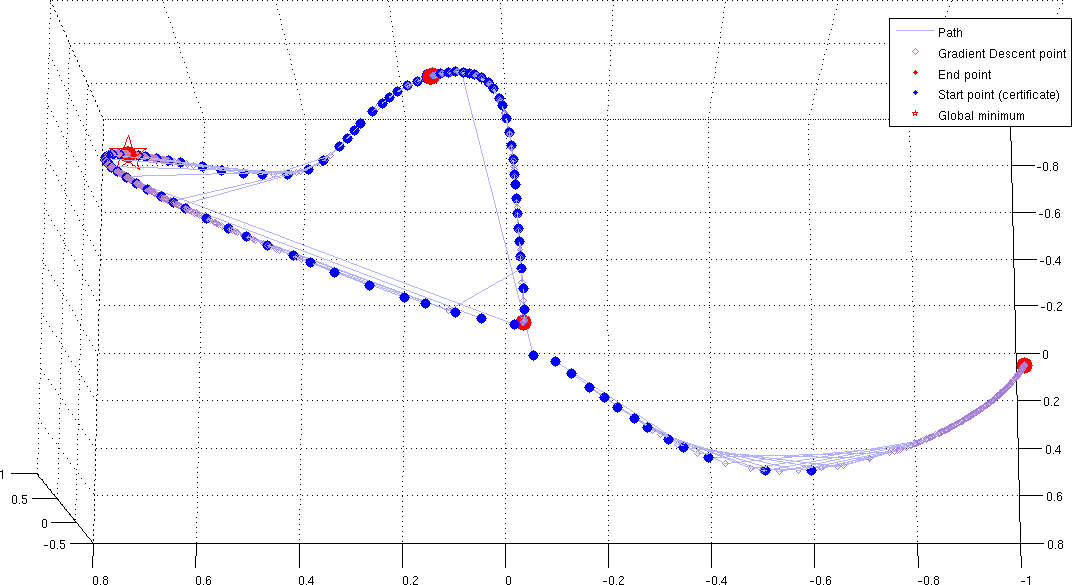
\includegraphics[height=60px]{example03_cbad_91pts_03.png}
\end{minipage}
\end{tabular}
\end{frame}
\begin{frame}{Results}
\centering 
\Huge Thank you!\\
Questions?
\end{frame}
\end{document} 